% !TEX encoding = UTF-8 Unicode
\documentclass[
10pt,
aspectratio=169,
]{beamer}
\setbeamercovered{transparent=10}
\usetheme[
  showheader,
%  red,
%  purple,
%  gray,
%  graytitle,
  colorblocks,
%  noframetitlerule,
]{Verona}

\usepackage[T1]{fontenc}
\usepackage[utf8]{inputenc}
\usepackage{lipsum}
\definecolor{col}{RGB}{0,68,158}
%%%%%%%%%%%%%%%%%%%%%%%%%%%%%%%
% Mac上使用如下命令声明隶书字体,windows也有相关方式,大家可自行修改
\providecommand{\lishu}{\CJKfamily{zhli}}
%%%%%%%%%%%%%%%%%%%%%%%%%%%%%%%
\usepackage{tikz}
\usetikzlibrary{shapes,
                tikzmark}
\tikzset{every tikzmarknode/.style={%
        semithick, inner sep=2pt}
        }


\usetikzlibrary{fadings}
%
%\setbeamertemplate{sections/subsections in toc}[ball]
\usepackage{xeCJK}
\usepackage{listings}
\usepackage{caption}
\usepackage{subcaption}
\usefonttheme{professionalfonts}
\def\mathfamilydefault{\rmdefault}
\usepackage{amsmath}
\usepackage{multirow}
\usepackage{booktabs}
\usepackage{bm}
\usepackage{mathtools}
\usepackage{algorithm}
\usepackage{algpseudocode}
\setbeamertemplate{section in toc}{\hspace*{1em}\inserttocsectionnumber.~\inserttocsection\par}
\setbeamertemplate{subsection in toc}{\hspace*{2em}\inserttocsectionnumber.\inserttocsubsectionnumber.~\inserttocsubsection\par}
\setbeamerfont{subsection in toc}{size=\small}
%\AtBeginSection[]{%
%	\begin{frame}%
%		\frametitle{Outline}%
%		\textbf{\tableofcontents[currentsection]} %
%	\end{frame}%
%}

\AtBeginSection[]{%
	\begin{frame}%
		\frametitle{A che punto stiamo}%
		\textbf{\tableofcontents[currentsection, currentsubsection]} %
	\end{frame}%
}

\title{Real time trackless beamline position\\ reconstruction at the LHCb experiment }
\subtitle{Tesi Ma Non Troppo}
\author[G.C.]{Giulio Cordova}
\mail{g.cordova@studenti.unipi.it}
\institute[Università di Pisa]{Dipartimento di Fisica E. Fermi\\
Università di Pisa}
\date{\today}
\titlegraphic[width=3cm]{cherubino_pant541}{}
%\definecolor{Veronagrayblue} {RGB}{0,91,129}
\newcommand\boldblue[1]{\textcolor{Veronagrayblue}{\textbf{#1}}}




%%%%%%%%%%%%%%%%%%%%%%%%%%%%%%%%
% ----------- 标题页 ------------
%%%%%%%%%%%%%%%%%%%%%%%%%%%%%%%%



\begin{document}

\maketitle


%%%%%%%%%%%%%%%%%%%%%%%%%%%%%%%%
% ----------- Temp ------------
%%%%%%%%%%%%%%%%%%%%%%%%%%%%%%%%

% \begin{exampleblock}{title}
% 		xxx
% 	\end{exampleblock}

% \begin{columns}[onlytextwidth]
% 		\begin{column}{.5\textwidth}
% 		\end{column}
% \end{columns}

% \begin{figure}
% 		\centering
% 		\includegraphics[width=0.8\linewidth]{fig/intro_private.png}
% 		\caption{Privacy security policy}
% \end{figure}

% \begin{equation*}
% 		w=\sum _{j=1}^{M}\frac{\left | \mathcal{D}_j \right | w_j^e}{\sum _{j=1}^{M}\left | \mathcal{D}_j \right |}
% \end{equation*}

%%%%%%%%%%%%%%%%%%%%%%%%%%%%%%%%
% ----------- FRAME ------------
%%%%%%%%%%%%%%%%%%%%%%%%%%%%%%%%


\section*{Overview}
\begin{frame}{Outline}
    \tableofcontents[]{}
\end{frame}
\section{Il percorso fino alla tesi}
\subsection{Triennale}
\begin{frame}{Triennale}
Laurea Triennale in Fisica a Pisa 
\vfill
Esami a scelta:
\begin{columns}
           \column{0.48\linewidth}
\begin{itemize}
    \item Astrofisica 
    \item Introduzione alla fisica subnucleare
\end{itemize}
\column{0.48\linewidth}
\begin{itemize}
    \item Mi è servito a capire che non mi piaceva
    \item Tonelli mi ha ipnotizzato
\end{itemize}
    \end{columns}
    \vfill
    Tesi triennale: Misure di preicisione del bosone W con l'esperimento CMS\\
    Relatore: Paolo Azzurri
    \vfill
    La tesi l'ho scelta insieme a Guido Tonelli alla fine del corso di fisica subnucleare. Tornassi indietro forse farei qualcosa di meno avanzato.
\end{frame}
\subsection{Magistrale}

\begin{frame}{Magistrale}
Curriculum: Data Analysis for Experimental Physics

    \begin{figure}
        \centering
        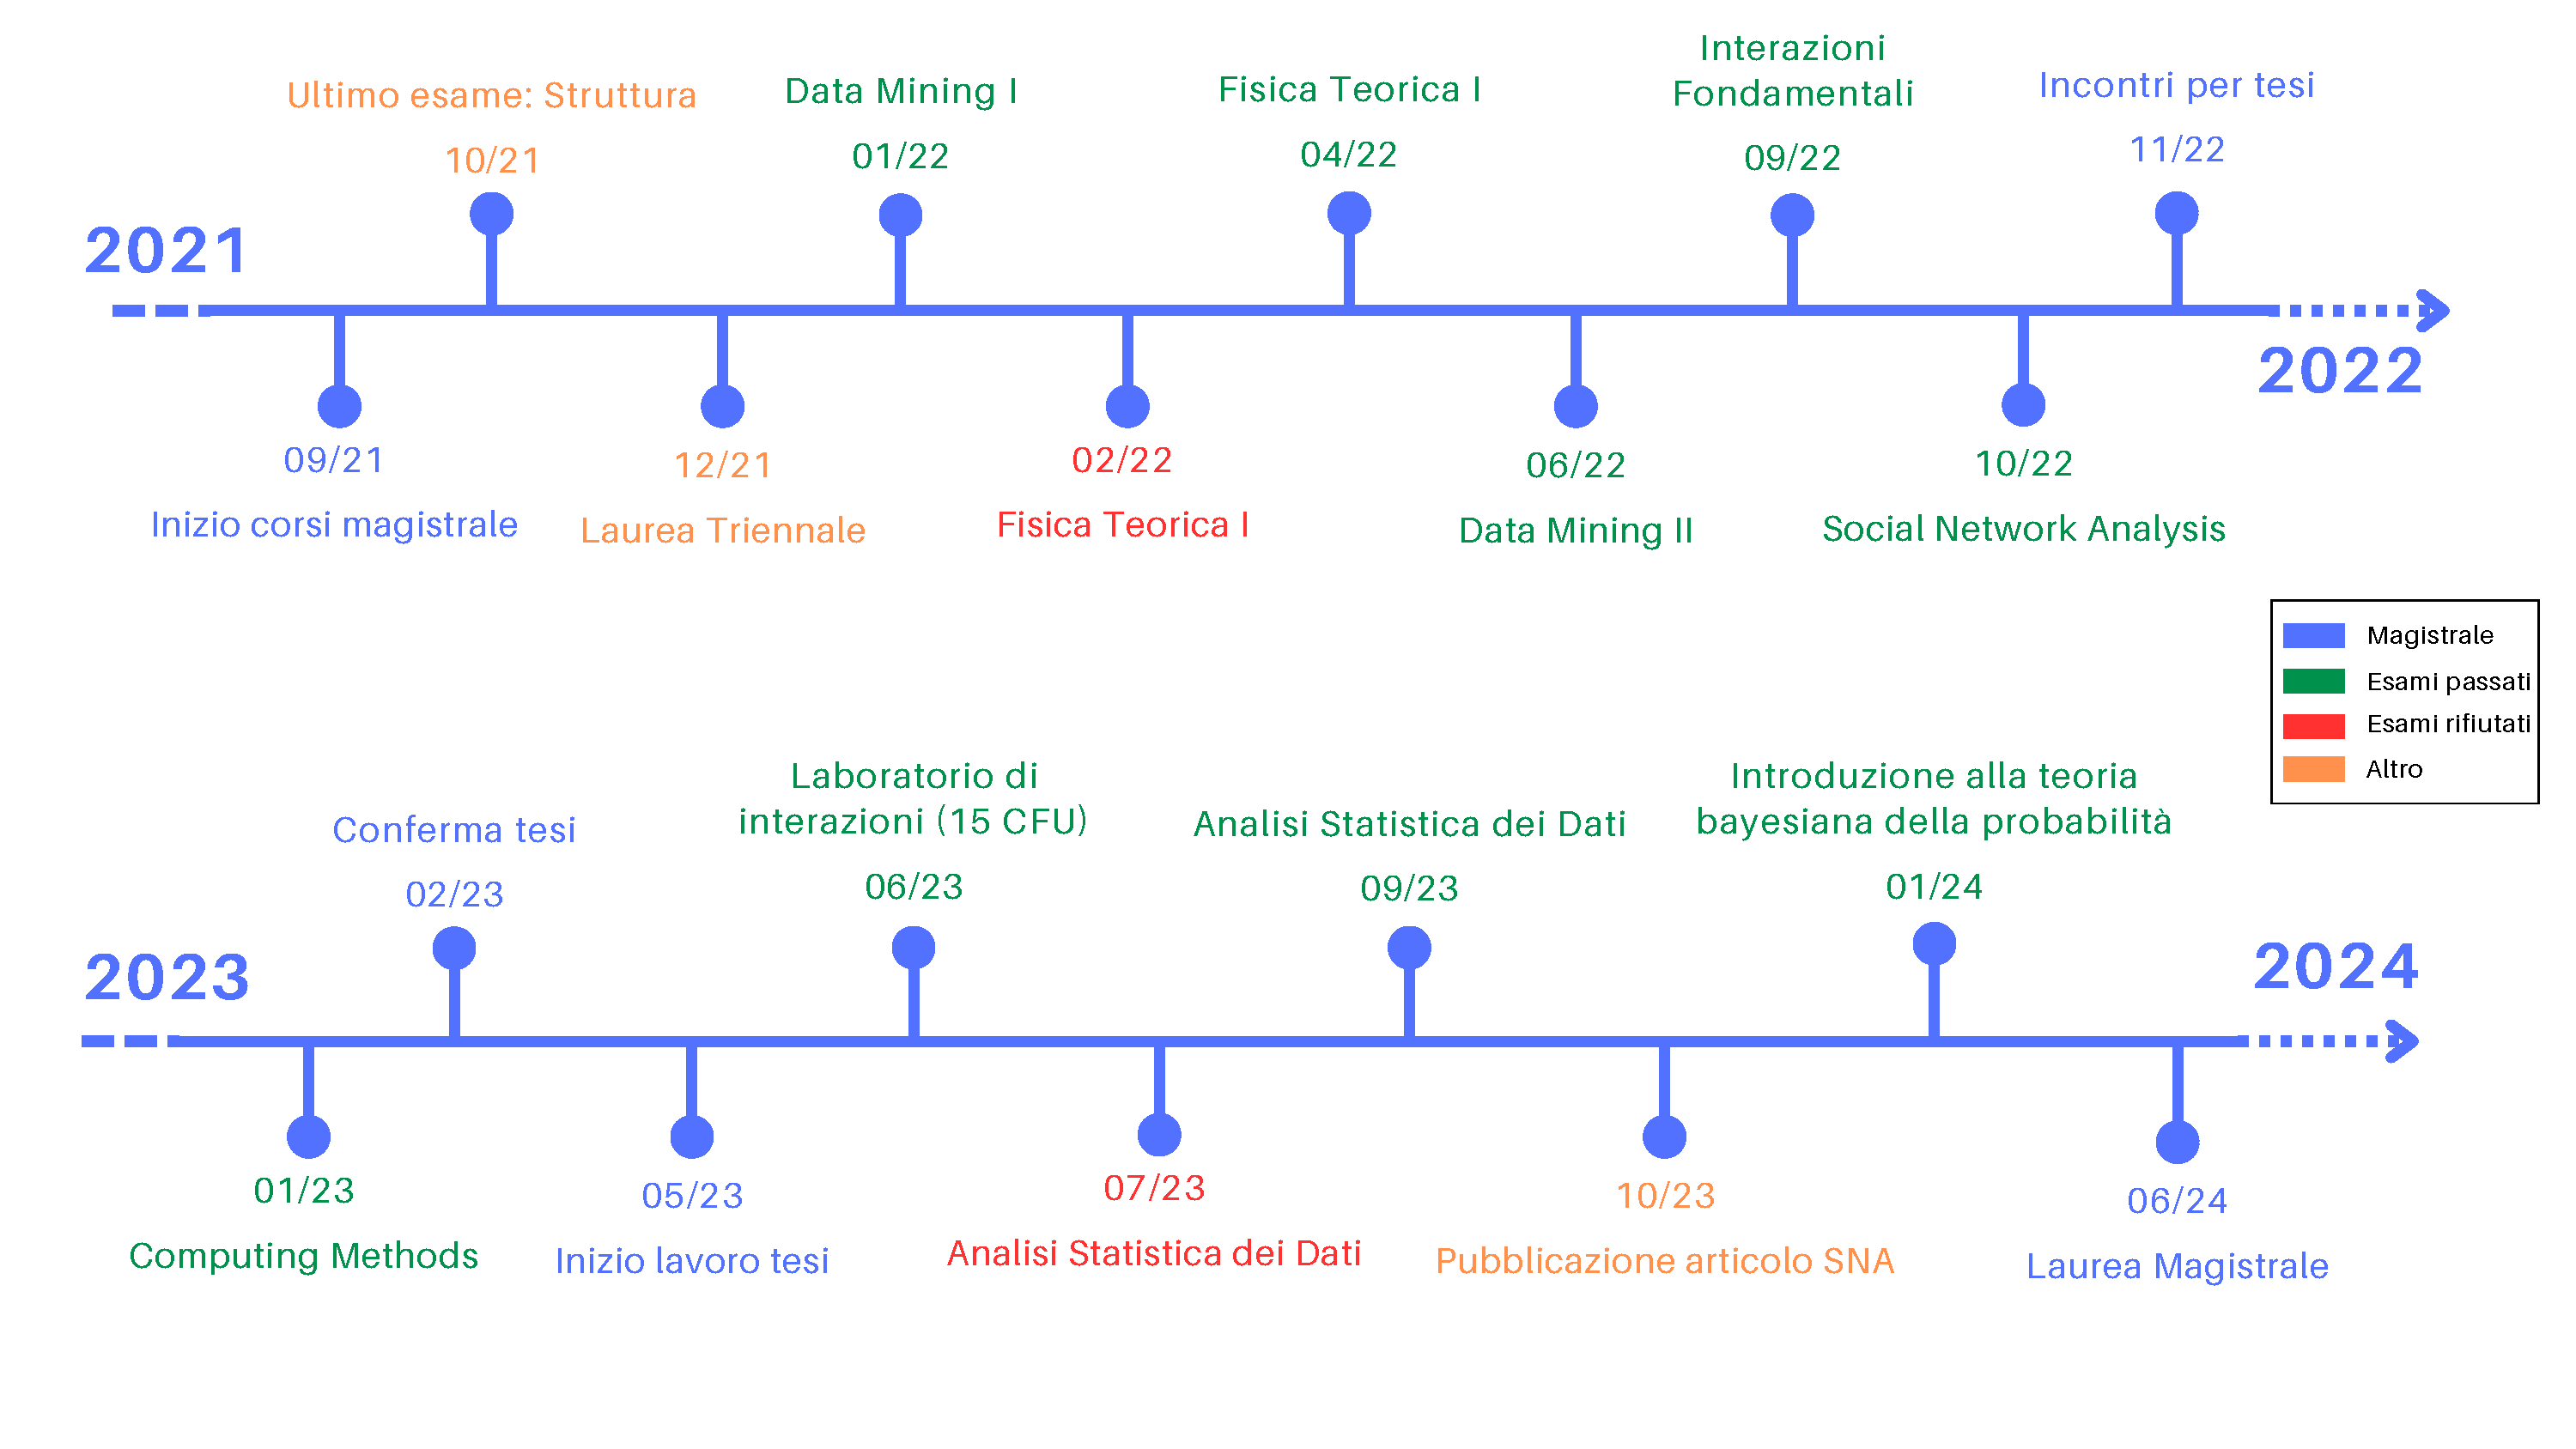
\includegraphics[width=0.93\textwidth]{timeline.pdf}
        %\caption{Caption}
        %\label{fig:enter-label}
    \end{figure}
\end{frame}

\begin{frame}[t]{Magistrale (fatta meglio)}
Se postessi ricominciare domani la magistrale la rifarei così:
\vfill
\begin{columns}[T]
    \column{0.48\linewidth}
    \textbf{Primo Anno:}
    \begin{itemize}
    \item Fisica Teorica 1 (gennaio)
    \item Interazioni Fondamentali (febbraio)
    \item Analisi Statistica dei Dati (aprile)
    \item Laboratorio di Interazioni Fondamentali (giugno)
    \item Data Mining (luglio)
    \item Computing Methods (fra settembre e dicembre)

    \end{itemize}
    \column{0.48\linewidth}
    \textbf{Secondo Anno:}
    \begin{itemize}
        \item Introduzione alla teoria bayesiana della probabilità (gennaio)
        \item Social Network Analysis (febbraio)
    \end{itemize}
\end{columns}
    \vfill
Meglio fare i corsi di indirizzo subito: io ho scoperto che mi piaceva stare in laboratorio e aggeggiare dopo aver già confermato la tesi... \\
In più meglio togliersi gli esami più difficili prima e tenersi quelli più facili in fondo!
    \end{frame}
\subsection{Come ho scelto la tesi}
\begin{frame}{Come ho scelto la tesi}
Ho parlato con un po' di persone.
\begin{itemize}
    \item Prof. Forti per un'idea sui vari esperimenti dell'area Interazioni Fondamentali
    \item Prof. Roda per l'esperimento ATLAS
    \item Prof. Donati per gli esperimenti a Fermilab
    \item \textbf{Prof. Punzi per l'eperimento LHCb}
    \item Prof. Casarosa per l'esperimento Belle II
    \item Prof. Azzurri per l'esperimento CMS
\end{itemize}
\vfill
Fun Fact: all'inizio Punzi mi aveva proposto un altro lavoro e lo stavo scartando, mi ha ricontattato successivamente perché gli era venuta un'altra idea più in linea con il mio percorso di studi.
\end{frame}
\section{Il lavoro di tesi}
\subsection{Il CERN e LHC}
\begin{frame}{Il CERN e il Large Hadron Collider}
Il CERN è una collaborazione internazionale e ha diversi esperimenti nella sua facility. I più famosi sono i quattro posti lungo il Large Hadron Collider (LHC), ma ne esistono molti altri!
\begin{figure}
    \centering
    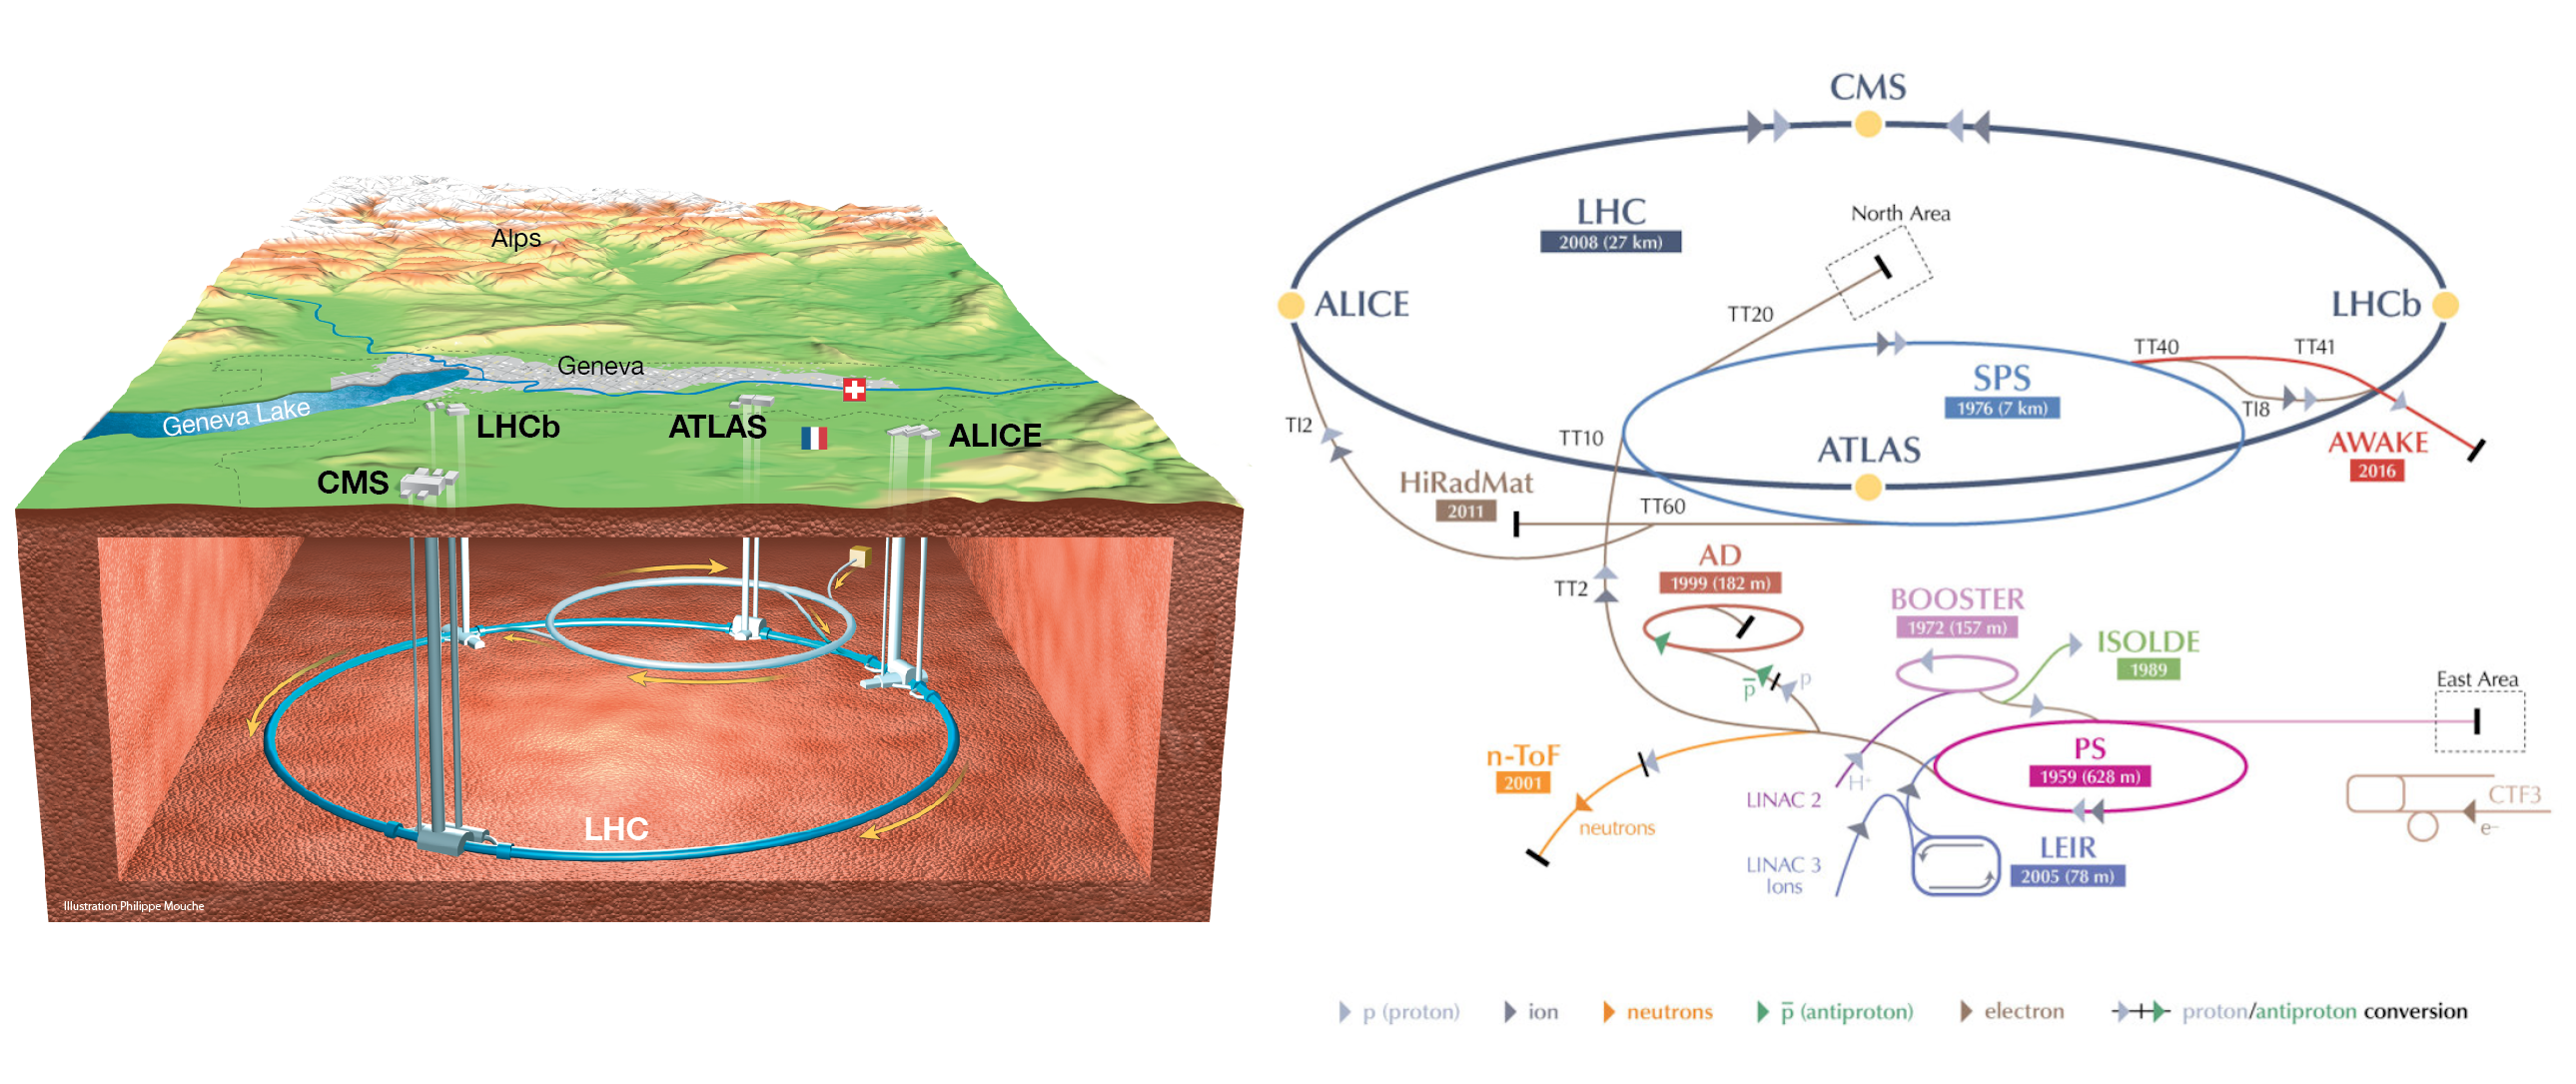
\includegraphics[width=0.8\linewidth]{lhc.png}
    %\caption{Caption}
    %\label{fig:enter-label}
\end{figure}
    LHC è un tunnel di 27 km dove vengono scontrati protoni a 14 TeV, al suo interno ha quattro caverne, per quattro esperimenti con scopi diversi: ATLAS, CMS, LHCb e ALICE
\end{frame}
\subsection{L'esperimento LHCb}
\begin{frame}{L'esperimento LHCb}
LHCb è un esperimento che studia quella che si chiama  fisica di sapore (flavour).\\
Il flavour delle particelle è un insieme di numeri quantici con cui si distinguono quark e leptoni.
\vfill
LHCb ha lo scopo di misurare i parametri della violazione della simmetria CP (parità e coniugazione di carica) e i decadimenti e fenomeni rari relativi agli adroni in cui è presente il quark beauty (quark b), da cui il nome dell'esperimento.  
\vfill
\begin{columns}
    \column{0.68\linewidth}
    Alcuni dei risultati più importanti di LHCb:
\begin{itemize}
    \item scoperta del decadimento ${\displaystyle B_{s}^{0}\to \mu ^{+}\mu ^{-}}$
\item scoperta del pentaquark (fun fact: non era nemmeno in programma per LHCb di scoprirlo)
\item violazione della simmetria di Carica-Parità nei mesoni D 
\end{itemize}
    \column{0.3\linewidth}
    \begin{figure}
        \centering
        
\includegraphics[width=\textwidth]{Lhcb-logo-new.png}
        %\caption{Caption}
        %\label{fig:enter-label}
    \end{figure}
\end{columns}
\vfill
Ti interessa sapere di più sul flavour delle particelle? Segui Interazioni Fondamentali e Fisica delle Particelle (e Cromodinamica Quantistica se proprio ti vuoi male)
\end{frame}

\begin{frame}{Il rivelatore di LHCb}
A differenza di tutti gli altri esperimenti al CERN, LHCb non è un rivelatore "a cipolla".
\begin{figure}
    \centering
    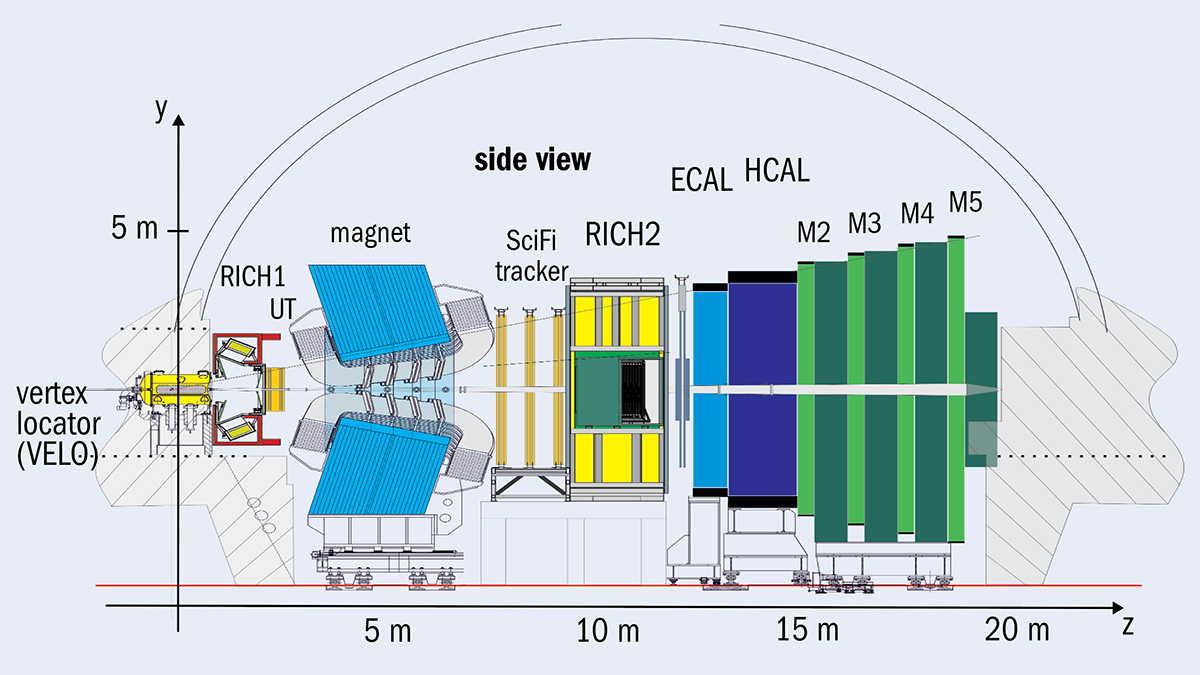
\includegraphics[width=0.7\textwidth]{detector.jpeg}
   % \caption{Caption}
    %\label{fig:enter-label}
\end{figure}    
Se ti interessano i rivelatori segui il corso di Instrumentation for Fundamental Physics di Forti.
\end{frame}

\begin{frame}{Dove lavoro io: il VELO}
    Rivelatore a pixel: sappiamo dove passa la particella in due coordinate x e y\\
    Composto da 26 stazioni (52 moduli, 26 sul lato A e 26 sul lato C)
    \begin{figure}
        \centering
        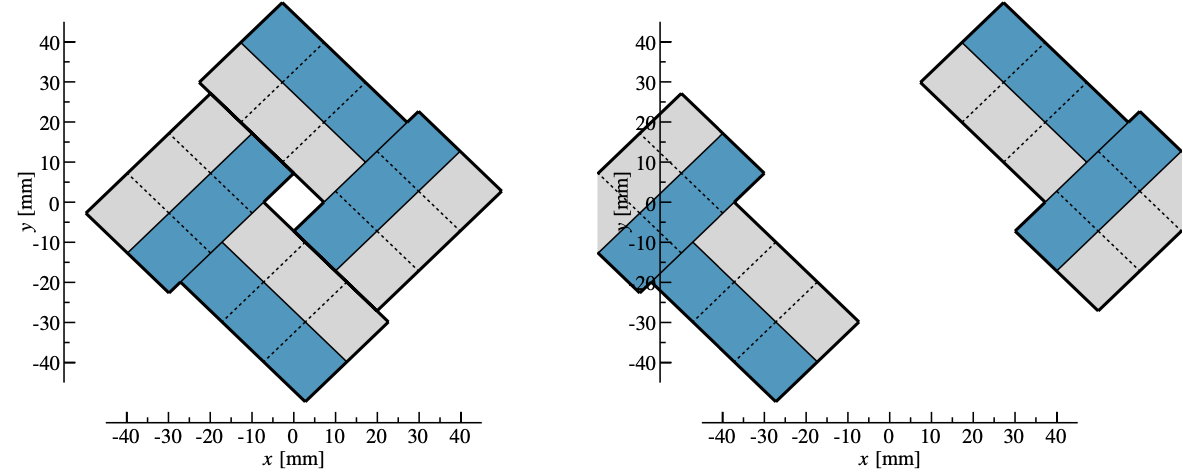
\includegraphics[width=0.48\textwidth]{aperture.png}
        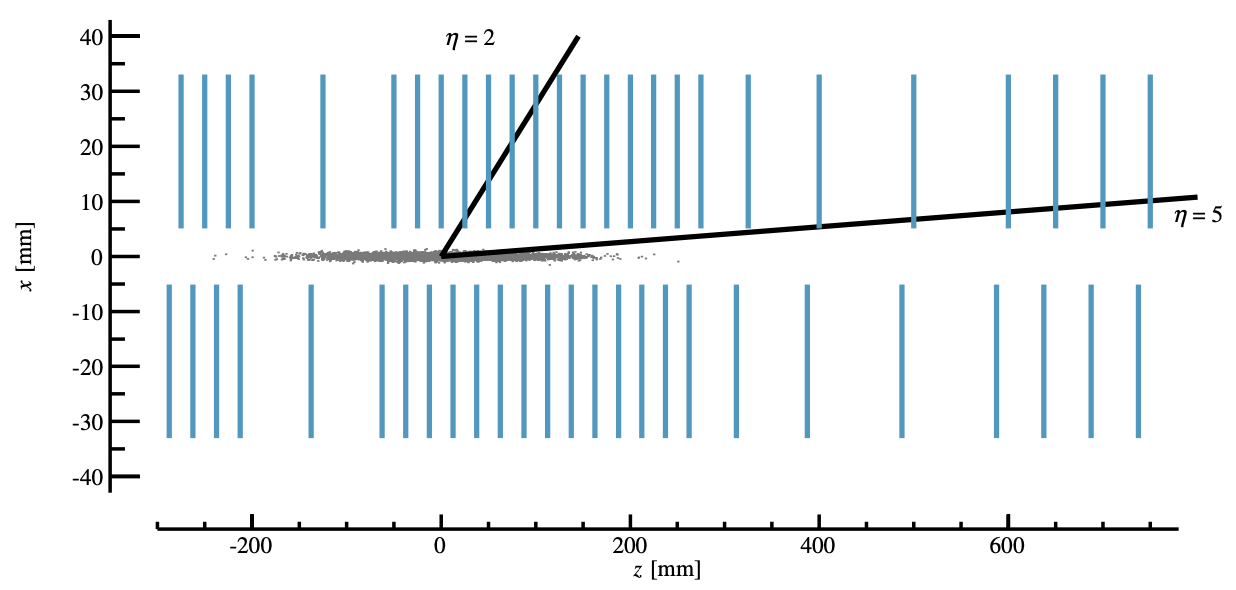
\includegraphics[width=0.5\textwidth]{above_view.png}
        %\caption{Caption}
        %\label{fig:enter-label}
    \end{figure}
    \vfill
    Cos'è un rivelatore a pixel, perché si usa il silicio sono tutte domande a cui troverete risposta nei corsi di "Introduzione alla Fisica Subnucleare", "Laboratorio di Interazioni Fondamentali" o "Instrumentation for Fundamental Physics"
\end{frame}

\begin{frame}{Il nuovo sistema di trigger di LHCb}
A LHC si ha una collisione ogni 25 nanosecondi (o 40 milioni di collisioni al secondo). Non tutte sono utili alle analisi che vogliamo fare. Vanno selezionate con un sistema trigger.
\begin{columns}
    \column{0.3\textwidth}
    \begin{figure}
        \centering
        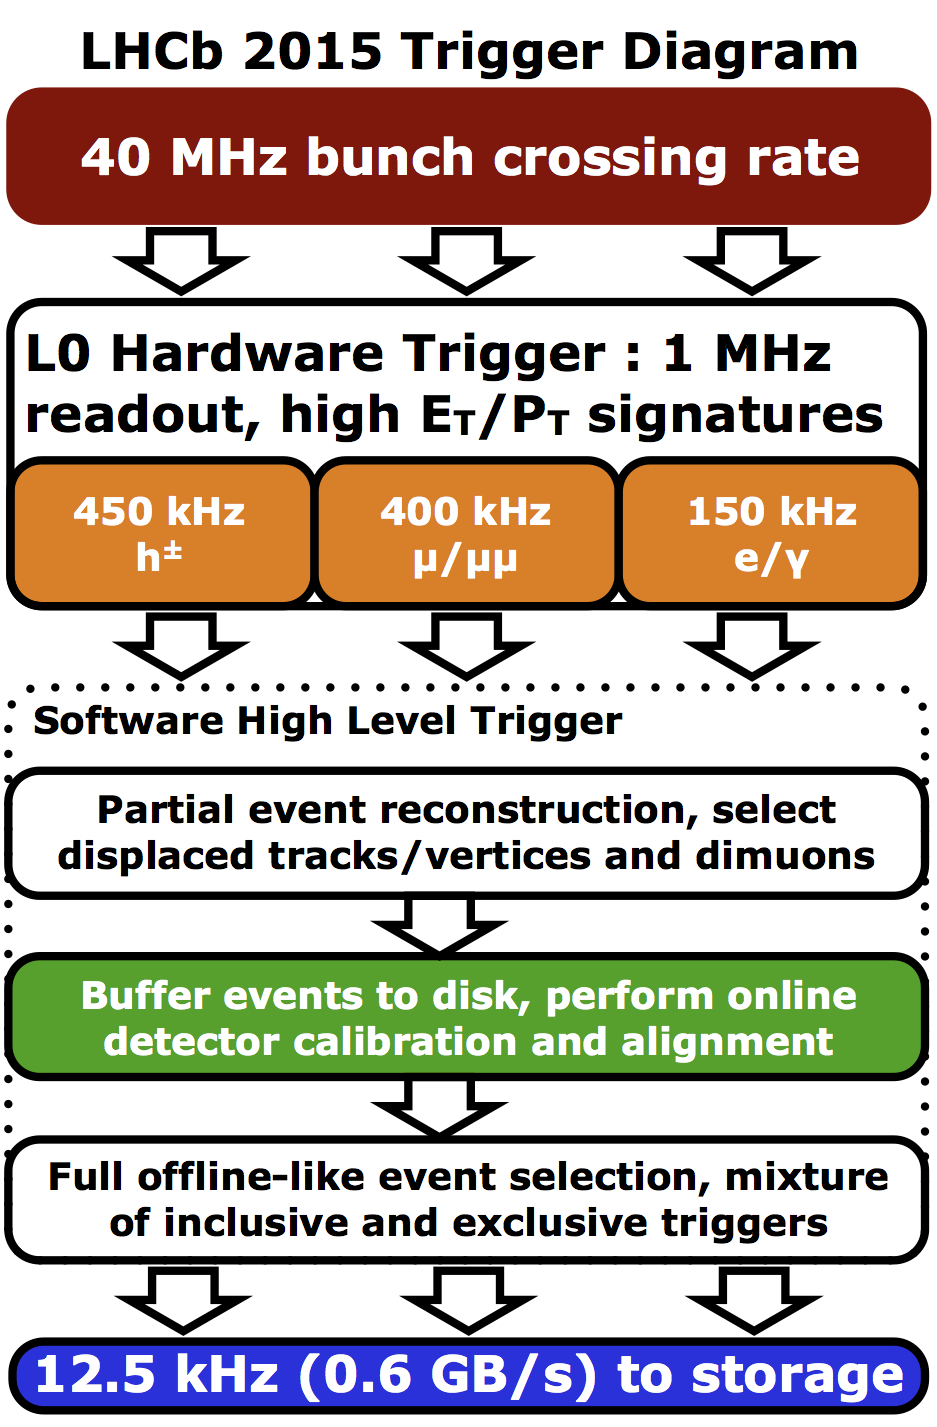
\includegraphics[width=0.9\linewidth]{LHCb_Trigger_RunII_May2015.jpeg}
        %\caption{Caption}
        %\label{fig:enter-label}
    \end{figure}
    \column{0.3\textwidth}
    \small
    Fino al Run II, il sistema di trigger era un misto fra hardware e software. Prima si fanno dei tagli con l'accetta guardando le informazioni dei rivelatori.
    
    \vspace{0.3cm}
    
    Dal Run III, LHCb ha detto fuck this, noi siamo superfighi e prima di buttare via eventi che ci potrebbero servire vogliamo esserne certi e hanno sviluppato un trigger software based in cui si ricostruisce l'intero evento in tempo reale.
    \column{0.3\textwidth}
    \begin{figure}
        \centering
        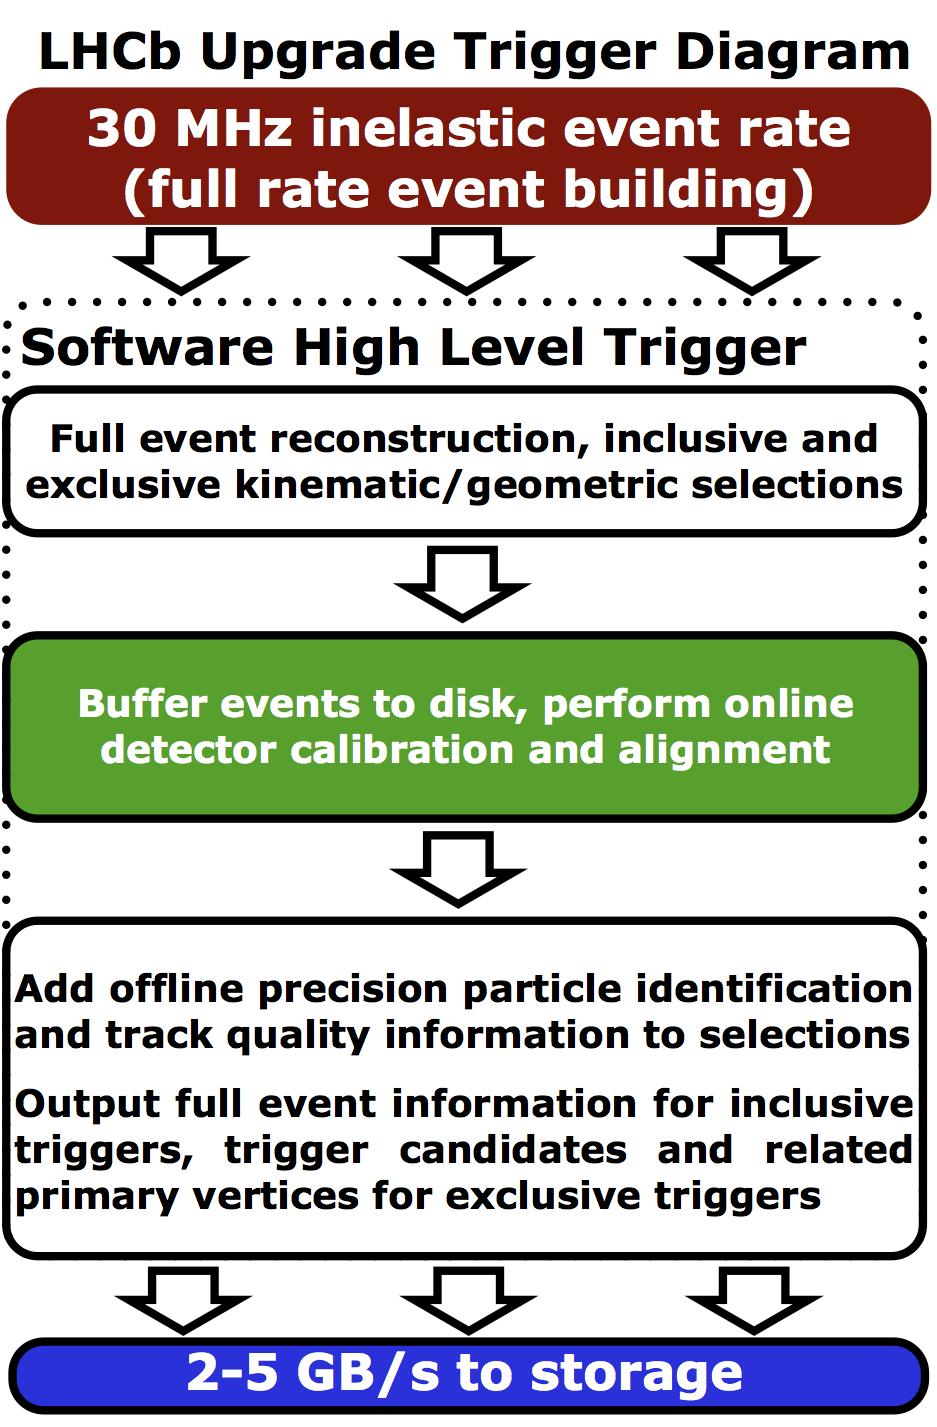
\includegraphics[width=0.9\linewidth]{LHCb_Trigger_RunIII_May2015.jpeg}
        %\caption{Caption}
        %\label{fig:enter-label}
    \end{figure}
\end{columns}
\end{frame}
\begin{frame}{La Real Time Analysis (RTA)}
La ricostruzione in tempo reale non è supportata dalle classiche CPU, ma bisogna dotarsi di sistemi di calcolo eterogeneo che permettono anche calcolo parallelo (GPU e FPGA).
\begin{figure}
    \centering
    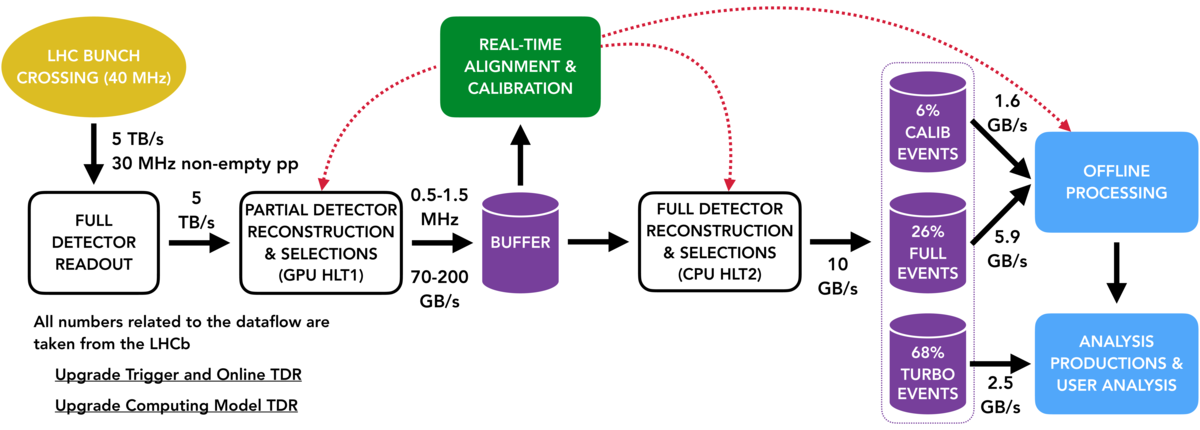
\includegraphics[width=\textwidth]{hidef_RTA_dataflow_widescreen.png}
    %\caption{Caption}
    %\label{fig:enter-label}
\end{figure}
    
\end{frame}
\begin{frame}{Che cosa si intende con beamline}
\begin{columns}
    \column{0.48\textwidth}
    A LHC si scontrano due fasci di particelle (blu e rosso), e interagiscono in una certa zona nello spazio.\\
    \vspace{0.5cm}
    Questa zona si chiama regione di luminosità (luminosity region) e corrisponde alla zona nera nella figura a destra. Da questa regione "escono" le particelle che noi analizziamo.\\

    \column{0.58\textwidth}
\begin{figure}
    \centering
    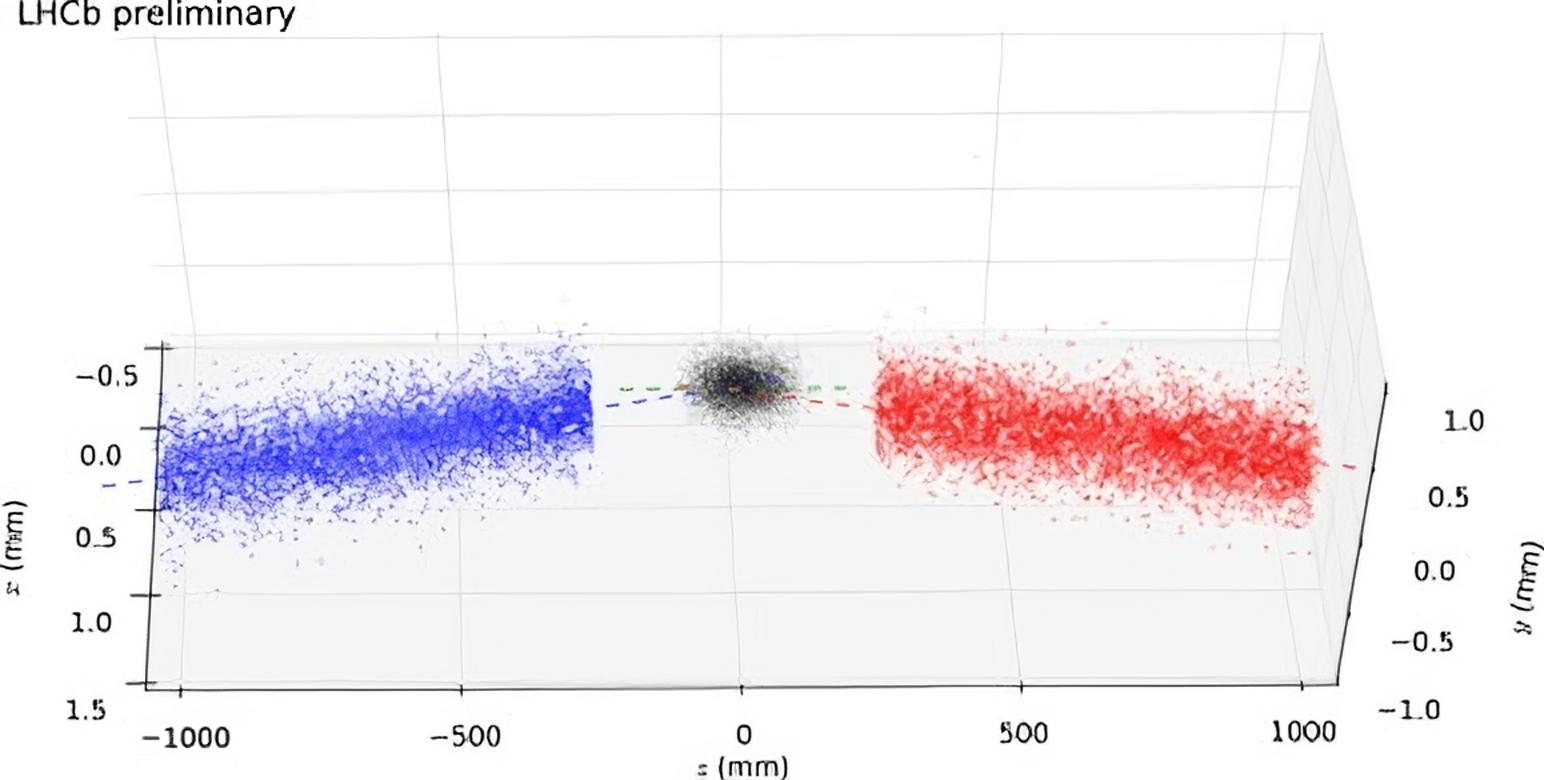
\includegraphics[width=\textwidth]{bgi-transformed.jpeg}
    %\caption{Caption}
    %\label{fig:enter-label}
\end{figure}
    \end{columns}

\end{frame}

\begin{frame}{Ricostruzione offline della beamline}
    Offline riusciamo a ricostruire questa regione con ottima precisione. 
    \begin{columns}
        \column{0.48\textwidth}
    \begin{itemize}
        \item Prima guardiamo le \textcolor{blue}{hit} delle particelle "figlie"
        \item Unendo i puntini delle \textcolor{blue}{hit} e altre informazioni del detector ricostruiamo le \textcolor{red}{tracce}
        \item Guardando il punto di origine delle varie \textcolor{red}{tracce} capiamo dove stava la beamline
    \end{itemize}
    \column{0.5\textwidth}

    \begin{figure}
        \centering
        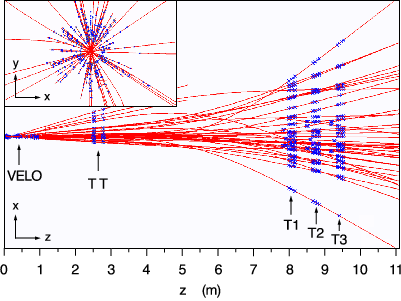
\includegraphics[width=\textwidth]{lots_of_tracks.png}
        %\caption{Caption}
        %\label{fig:enter-label}
    \end{figure}
        \end{columns}
Gli algoritmi di ricostruzione delle tracce però hanno bisogno come input la posizione della beamline!
È un processo iterativo molto lungo e complicato...
\end{frame}
\subsection{I miei due centesimi}
\begin{frame}{Contatori sul VELO}
    Idea: anziché usare le tracce partiamo direttamente dai cluster di hit sul VELO.
    \begin{columns}
        \column{0.48\textwidth}
        \begin{itemize}
            \item Definiamo delle regioni di selezione in zone specifiche del VELO
            \item Se mettiamo 8 regioni in ogni stazione abbiamo 208 contatori (ho 26 stazioni)
            \item Contiamo quanti cluster di hit cadono in ognuna di queste regioni di selezione
            \item Posso combinare l'informazione di questi 208 contatori per ottenere una stima della posizione della beamline?
        \end{itemize}

        \column{0.48\textwidth}
        \begin{figure}
            \centering
            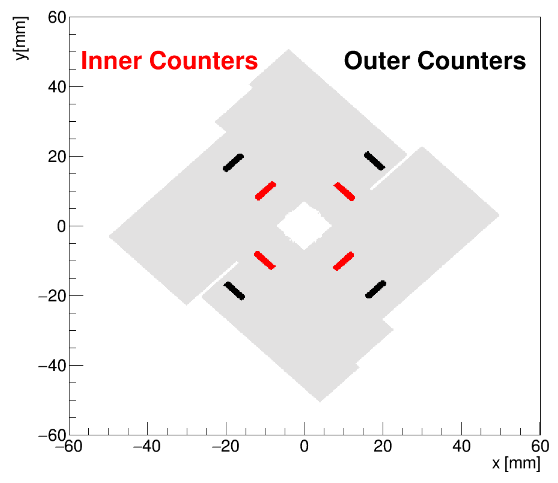
\includegraphics[width=\textwidth]{counters.png}
            %\caption{Caption}
            %\label{fig:enter-label}
        \end{figure}
    \end{columns}
\end{frame}



\begin{frame}{Principal Component Analysis (PCA)}
    La PCA è una trasformazione ortogonale lineare per un nuovo set di coordinate  tale per cui
    \begin{columns}
    \column{0.48\textwidth}
    \begin{itemize}
        \item La proiezione dei dati sulla prima componente trasformata ha la varianza più grande rispetto a tutte le altre proiezioni
        \item La proiezione dei dati sulla seconda componente trasformata ha la seconda varianza più grande ed è perpendicolare alla prima componente
        \item e così via
    \end{itemize}
    \column{0.48\textwidth}
    \begin{figure}
        \centering
        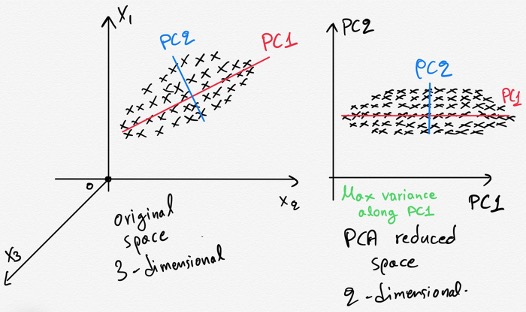
\includegraphics[width=\textwidth]{pca.jpg}
        %\caption{Caption}
        %\label{fig:enter-label}
    \end{figure}
\end{columns}
\vfill
Rimemebranze di geometria? Per proiettare i dati lungo una componente basta fare un prodotto scalare, che è un operazione semplice e veloce da eseguire!\\
La componente k-esima sarà quindi data da  $f_k = \vec{x}\vec{w_k}$, dove $\vec{x}$ sono i  dati e $\vec{w_k}$ un vettore di pesi da determinare con la PCA.
\end{frame}

\begin{frame}{Come determinare questo vettore}
I 208 contatori a disposizione formano una base per uno spazio 208-dimensionale. 
\vfill
Se avessimo un dataset in cui l'unico parametro che cambia nei dati fosse proprio la posizione della beamline lungo una direzione, possiamo calcolare le componenti principali.
\vfill
Questa è cosa che si fa facilmente con un Monte Carlo!
\vfill
Una volta che abbiamo il Monte Carlo applichiamo l'algoritmo che prevede banalmente la diagonilazzazione della matrice di covarianza
\begin{itemize}
    \item Gli autovettori trovati sono le componenti principali (la nuova base)
    \item Queste componenti principali sono ordinate in base agli autovalori
    \item Il k-esimo autovalore normalizzato corrisponde alla percentuale di varianza spiegata da quella componente
\end{itemize}

\end{frame}

\begin{frame}{Risultati su Monte Carlo}
Molto meglio delle aspettative, c'è una dipendenza lineare perfetta fra la prima componente stimata con la PCA e la posizione della beamline.\\
E si ha una risoluzione di 18 micrometri!
    \begin{columns}
    \column{0.5\textwidth}
        \begin{figure}
            \centering
            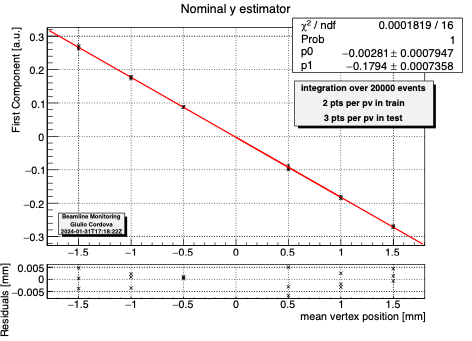
\includegraphics[width=\textwidth]{y_fit_MC.png}
            %\caption{Caption}
            %\label{fig:enter-label}
        \end{figure}
        \column{0.5\textwidth}
        \begin{figure}
            \centering
            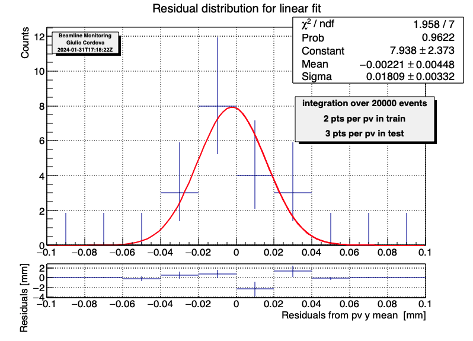
\includegraphics[width=\textwidth]{x_res_MC.png}
            %\caption{Caption}
            %\label{fig:enter-label}
        \end{figure}
    \end{columns}
\end{frame}

\begin{frame}{Dati reali}
E anche sui dati veri funziona! Ovviamente con una risoluzione leggermente peggiore, ma comunque nell'ordine di decine di micrometri.
        \begin{columns}
    \column{0.5\textwidth}
        \begin{figure}
            \centering
            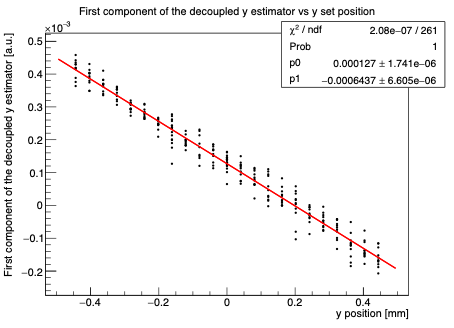
\includegraphics[width=\textwidth]{y_fit_dati.png}
            %\caption{Caption}
            %\label{fig:enter-label}
        \end{figure}
        \column{0.5\textwidth}
        \begin{figure}
            \centering
            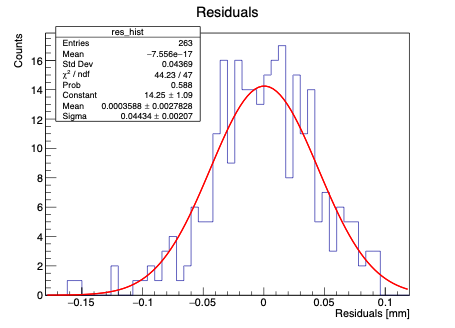
\includegraphics[width=\textwidth]{y_res_dati.png}
            %\caption{Caption}
            %\label{fig:enter-label}
        \end{figure}
    \end{columns}
\end{frame}

\begin{frame}{La bellezza di un lavoro sperimentale...}
Al momento sto investigando perché il mio stimatore funziona molto in una componente (y) e molto male nell'altra (x).
\vspace{-0.2cm}
    \begin{columns}
    \column{0.5\textwidth}
        \begin{figure}
            \centering
            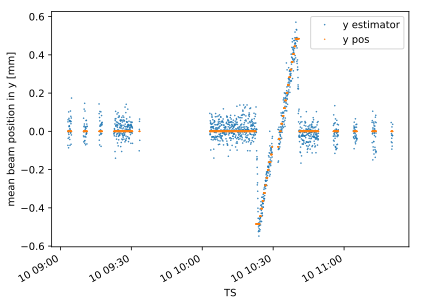
\includegraphics[width=\textwidth]{y_estimator.png}
            %\caption{Caption}
            %\label{fig:enter-label}
        \end{figure}
        \column{0.5\textwidth}
        \begin{figure}
            \centering
            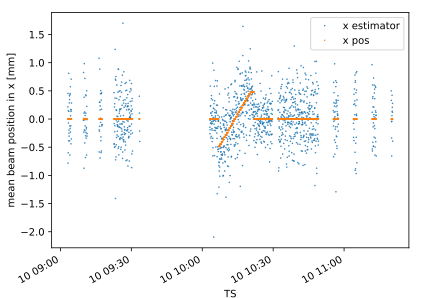
\includegraphics[width=\textwidth]{x_estimator.png}
            %\caption{Caption}
            %\label{fig:enter-label}
        \end{figure}
    \end{columns}
    \vfill
    Ma è proprio questo il bello di un lavoro sperimentale, che bisogna fronteggiare difficoltà che sulla carta non esistono, come contatori che non funzionano, link che si rompono, eccetera...
\end{frame}
\section{A contorno della tesi}
\subsection{Il gruppo di Pisa}
\begin{frame}{Il gruppo di Pisa}
    Al momento siamo il gruppo di LHCb più grande in Italia!
    Abbiamo:
    \begin{columns}
        \column{0.48\textwidth}
    \begin{itemize}
        \item 3 professori
        \begin{itemize}
            \item Prof. Giovanni Punzi
            \item Prof. Michael Joseph Morello
            \item Prof.ssa Elena Graverini
        \end{itemize}
        \item 6 ricercatori:
        \begin{itemize}
            \item John Walsh
            \item Matteo Rama
            \item Riccardo Fantechi
            \item Federico Lazzari
            \item Sergei Kholodenko
            \item Ao Xu
        \end{itemize}
        \end{itemize}
        \column{0.48\textwidth}
        \begin{itemize}
        \item 6 dottorandi
        \begin{itemize}
            \item Lorenzo Pica
            \item Francesco Terzuoli
            \item Nico Klejne
            \item Francesco Paciolla
            \item Domenico Riccardi
            \item Daniele Passaro
        \end{itemize}
        \item 2 studenti magistrali
        \begin{itemize}
            \item Irene Celestino
            \item Giulio Cordova
        \end{itemize}
    \end{itemize}
        \end{columns}
        \vfill
Come vedete anche da questi numeri LHCb non è un'esperimento grandissimo come potrebbe essere ATLAS o CMS. \\
Ma siamo comunque una collaborazione internazionale composta da 1692 persone provenienti da 22 paesi diversi!
\end{frame}
\subsection{Le cose belle}
\begin{frame}{Bilanci}
\begin{columns}
    \column{0.5\textwidth}
    Le cose belle:
\begin{itemize}
    \item Ho un ufficio all'INFN
    \item Sono tutti iperdisponibili
    \item Mi mandano in missione al CERN (già una volta e ci dovrei tornare a breve)
    \item Partecipo attivamente alla collaborazione
    \item LHCb è il gruppo con più vita sociale del CERN (barbecue, collaboration drinks, etc.)
    \end{itemize}
    \begin{figure}
        \centering
        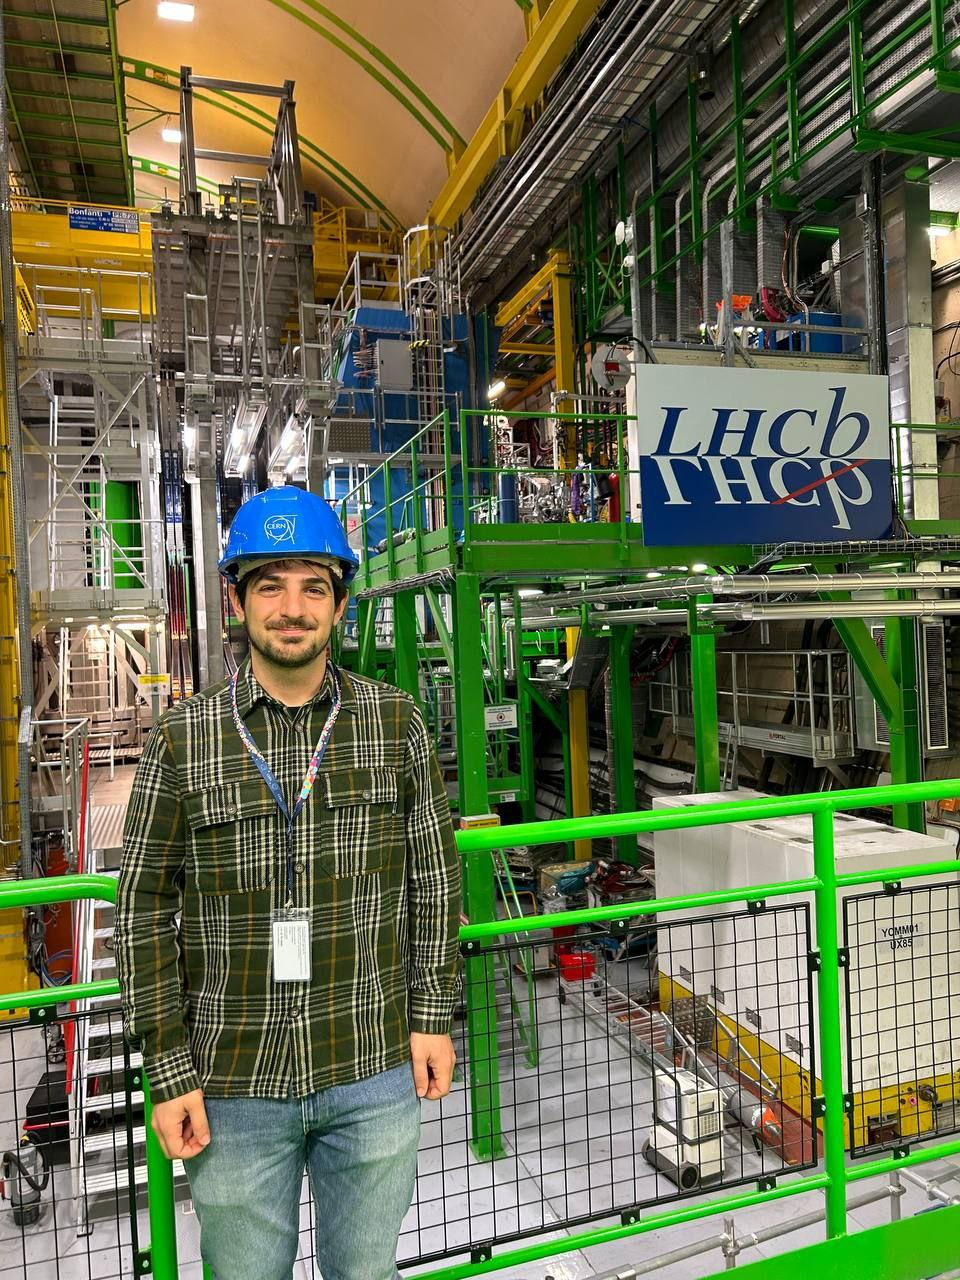
\includegraphics[width=0.3\textwidth]{caverna.jpeg}
                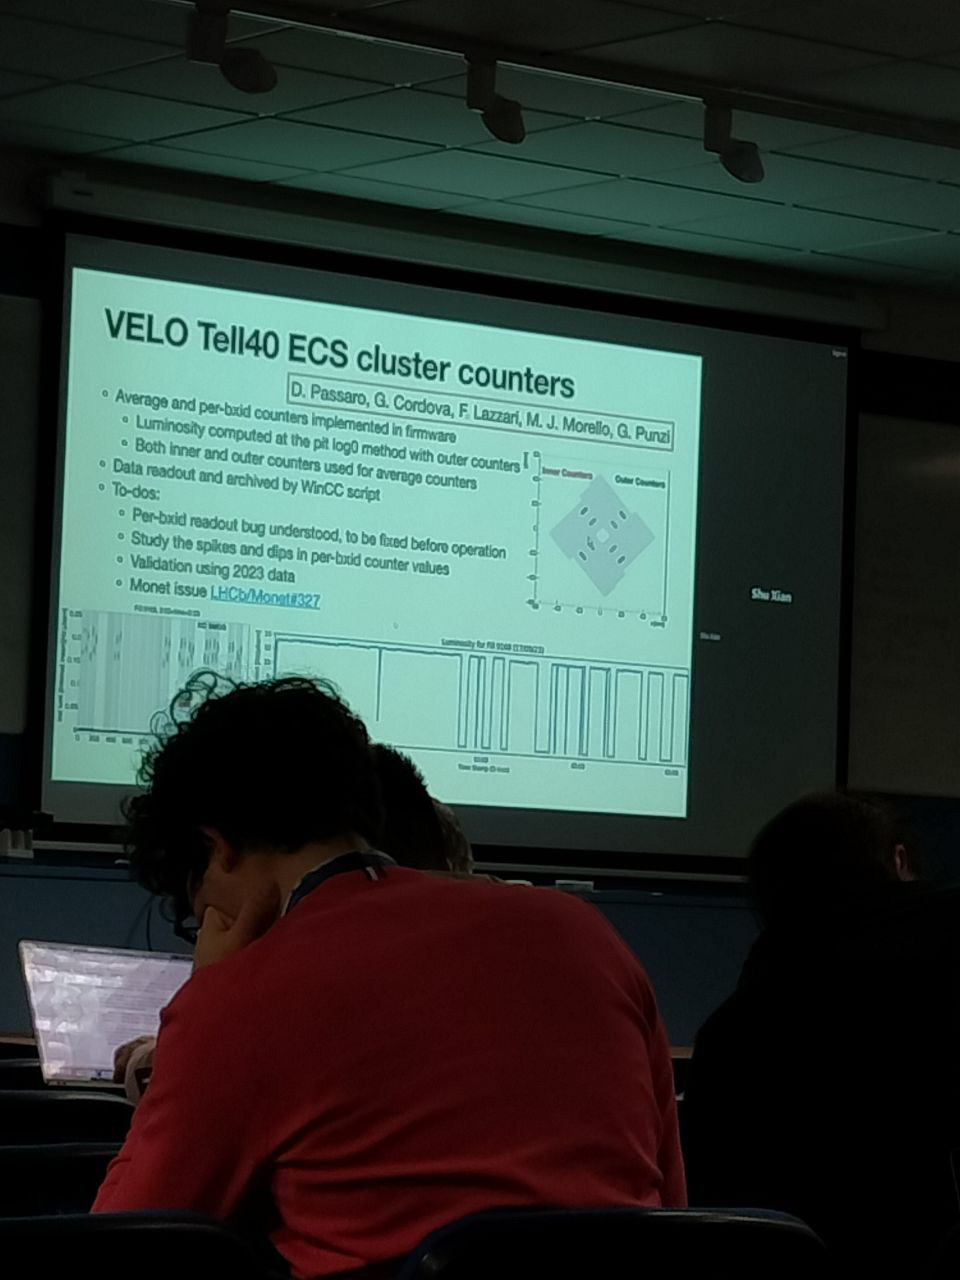
\includegraphics[width=0.3\textwidth]{mio_plot.jpeg}
        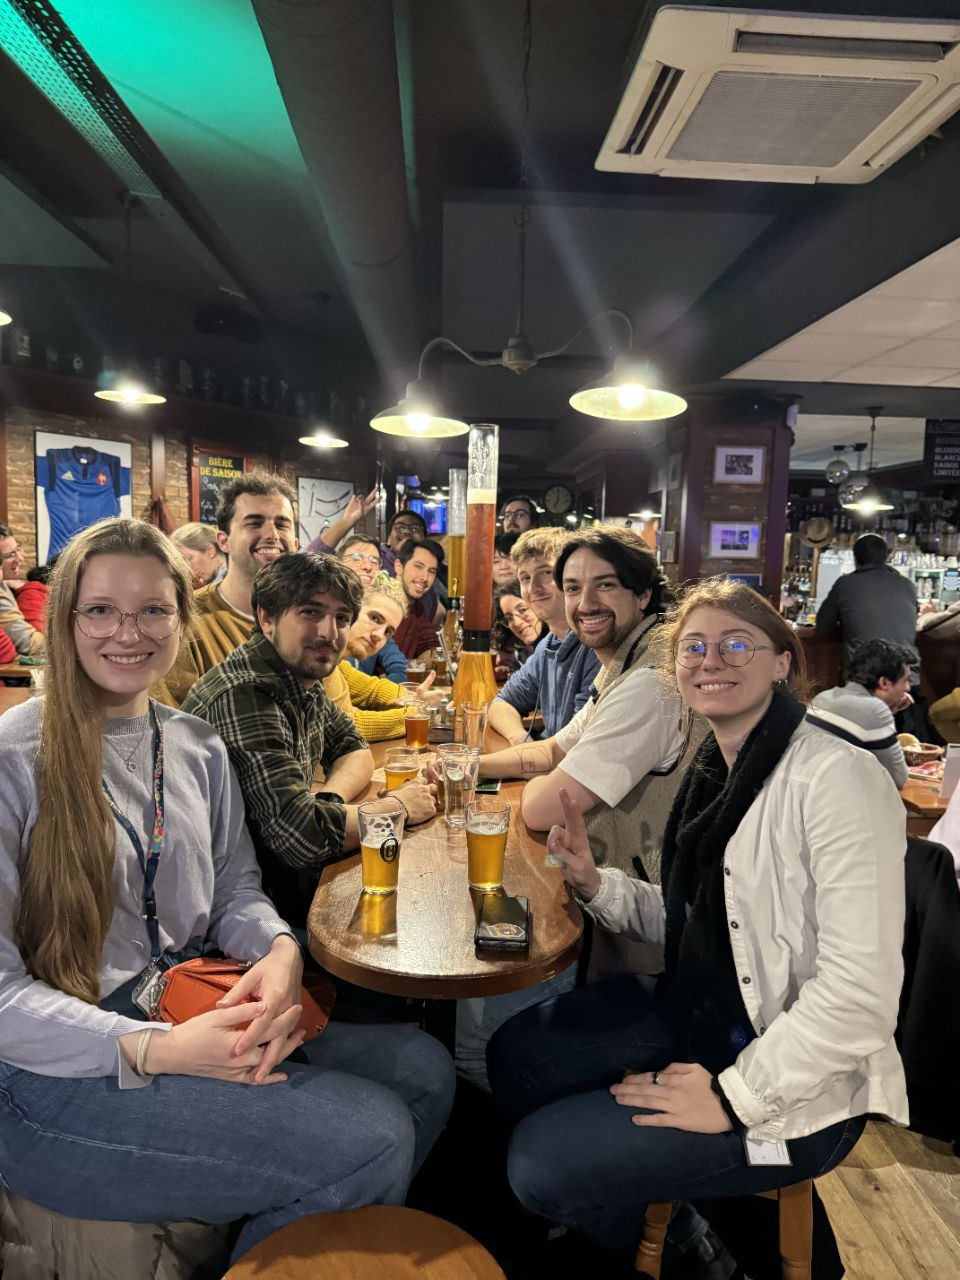
\includegraphics[width=0.3\textwidth]{birra.jpeg}

        %\caption{Caption}
        %\label{fig:enter-label}
    \end{figure}
    \column{0.5\textwidth}
    Le cose meno belle:
    \begin{itemize}
    \item Il lavoro richiesto è molto (ma anche appagante)
    \item L'esperimento si trova in una fase critica 
    \item Il relatore è molto impegnato e spesso non raggiungibile
    \item Il lavoro di tesi è un po' lungo
\end{itemize}
\begin{figure}
        \centering
        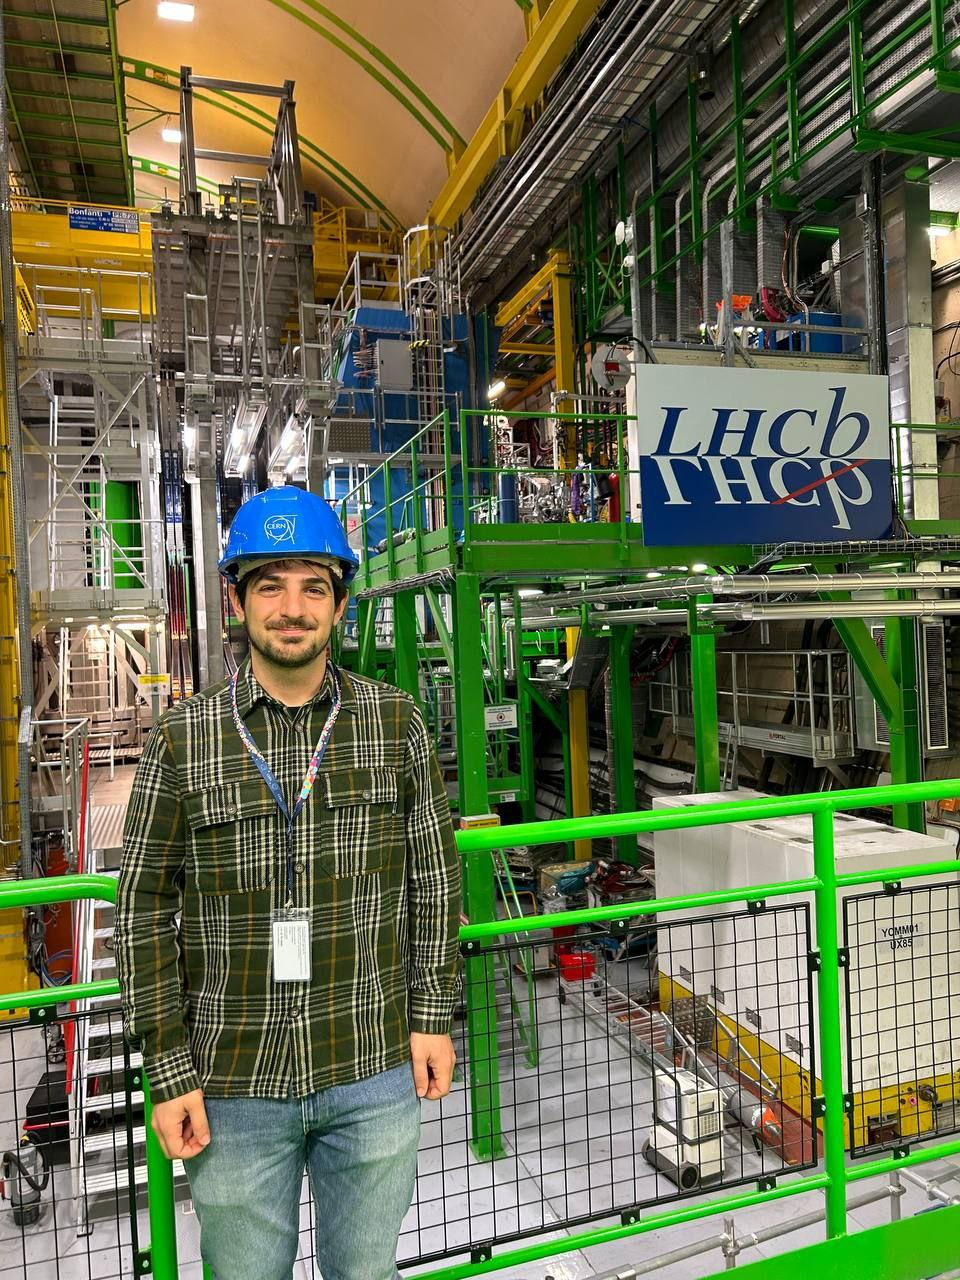
\includegraphics[width=0.3\textwidth]{caverna.jpeg}
                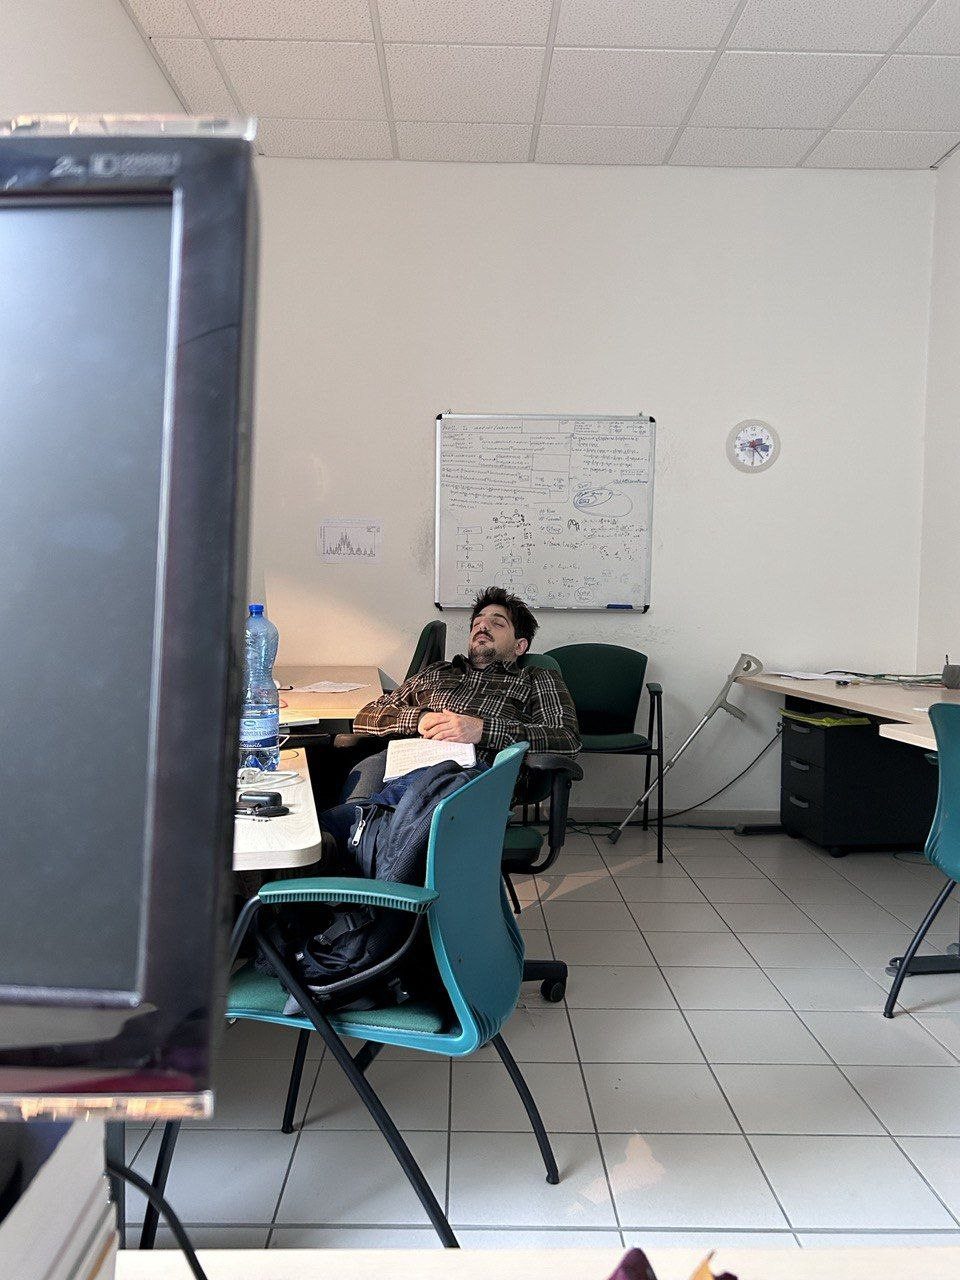
\includegraphics[width=0.3\textwidth]{ufficio.jpeg}
        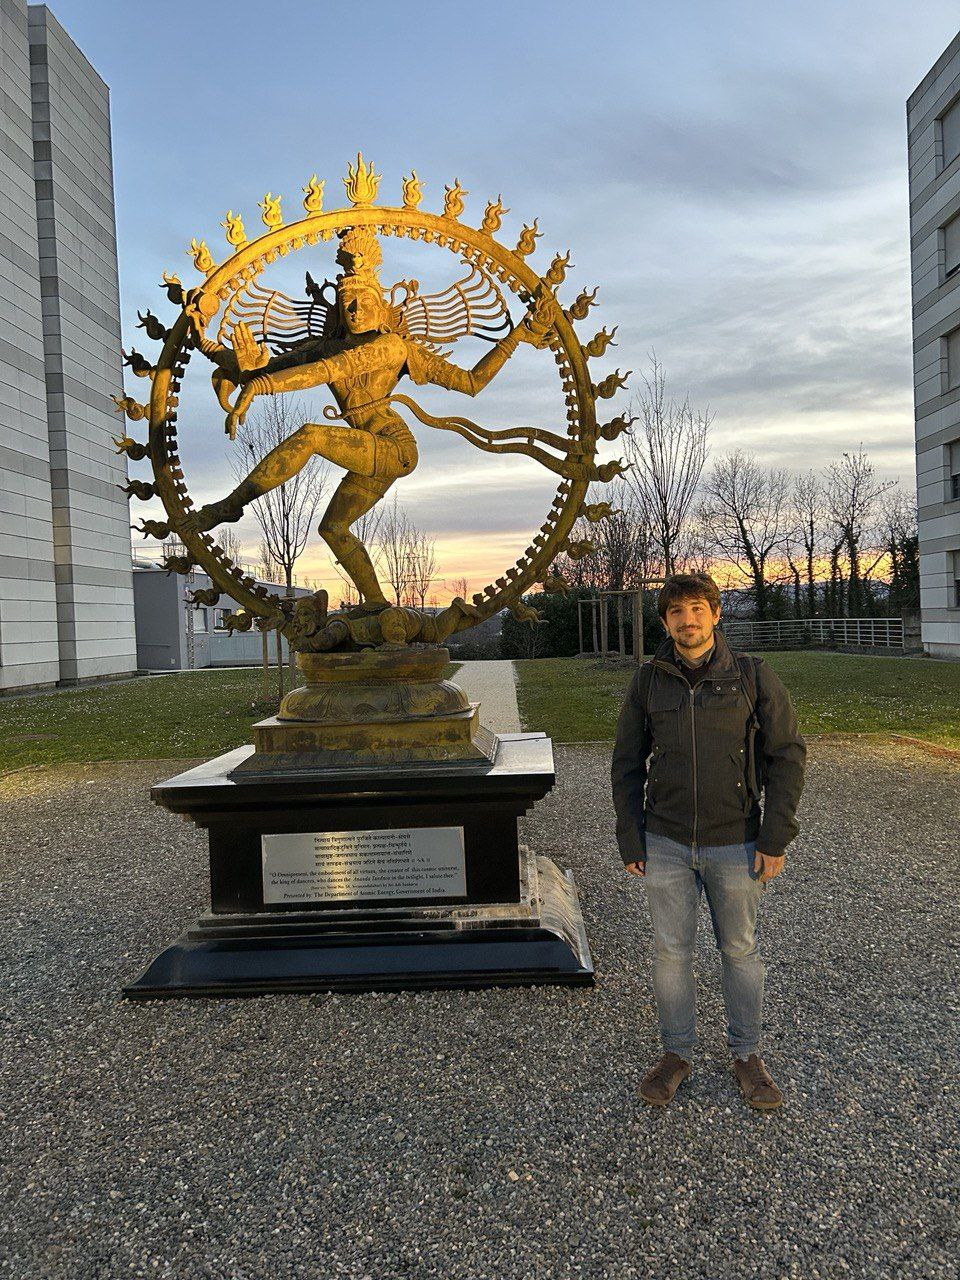
\includegraphics[width=0.3\textwidth]{shiva.jpeg}

        %\caption{Caption}
        %\label{fig:enter-label}
    \end{figure}
\end{columns}
\end{frame}
\subsection{Le cose meno belle}


\begin{frame}{Sum up}
\begin{itemize}
    \item Lavorare a una tesi al CERN è molto bello!
    \item Dal mio punto di vista, LHCb è un buon equilibrio fra collaborazione internazionale e dimensione del gruppo
    \item Nella mia magistrale cambierei un po' di cose, ma gli esami fatti mi hanno fornito una base solida
    \item Il relatore riesce a trasmettere passione e a stimolarti per dare sempre di più
    \item Il gruppo è molto gentile e ognuno è sempre disponibile a darti una mano
    \item Il lavoro che ho fatto è stato soddisfacente, ma di fisica ho visto poco
    \item Ho portato a casa dei risultati importanti per la collaborazione e spero che possano aiutarla in questa fase critica
\end{itemize}
    
\end{frame}

\beamertemplateshadingbackground{structure.fg!90}{structure.fg}
\begin{frame}[plain]
	\vfill
	\centering
	{
		\centering \Huge \color{white} Grazie per l'attenzione!%\\[10pt]Questions?
	}
	\vfill
\end{frame}
\end{document}